\documentclass[a4paper]{article}

\usepackage[per-mode=symbol,separate-uncertainty=true]{siunitx}
\usepackage{amsmath}
\usepackage{float}
\usepackage{graphicx}
\usepackage[a4paper,top=3cm,bottom=2cm,left=3cm,right=3cm,marginparwidth=1.75cm]{geometry}
\usepackage{mathtools}
\usepackage{siunitx}
\usepackage[colorlinks=true, allcolors=blue]{hyperref}
\usepackage[dvipsnames]{xcolor}

\sisetup{exponent-product=\cdot}

\title{Integrated System Architecture \\ Lab session 3 report - RISC-V special project}
\author{Marco Andorno (247222)\\ Michele Caon (253027) \\ Alessio Colucci (251197) \\ Matteo Perotti (251453) \\ Giuseppe Sarda (255648)}

\begin{document}
\maketitle
\tableofcontents

\section{Introduction}
The aim of this laboratory session is to design a simple RISC-V core implementing the RV32I instruction set in SystemVerilog, which is the basic 32-bit integer-only set of instructions, without multiply and divide. The complete set is shown in figure \ref{fig:rv32i}.

\begin{figure}[hbtp]
    \centering
    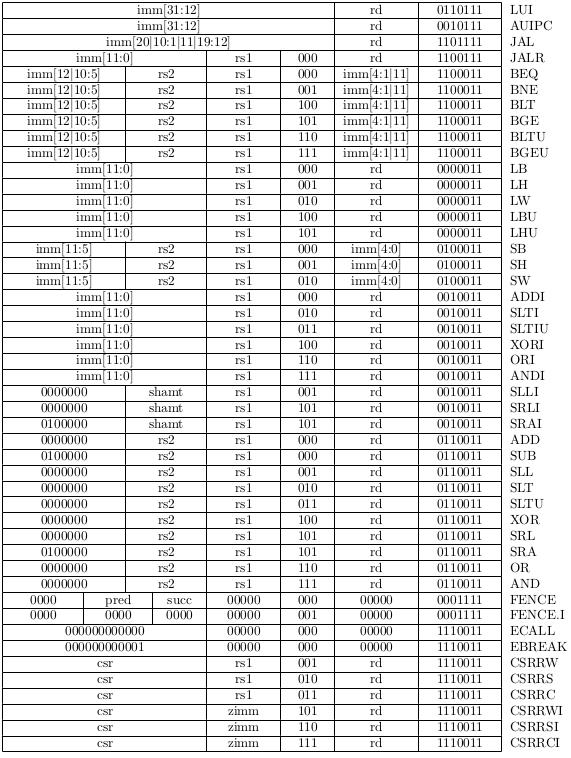
\includegraphics[width=.8\textwidth]{img/RISCV_RV32I_instr2.jpg}
    \caption{RV32I instructions}
    \label{fig:rv32i}
\end{figure}

Actually, not all the instructions were implemented as the support for an operating system and exception handling is beyond the scope of this experience.

The different formats of the instructions are shown in figure \ref{fig:formats}, which is useful reference in the rest of this report.

\begin{figure}[hbtp]
    \centering
    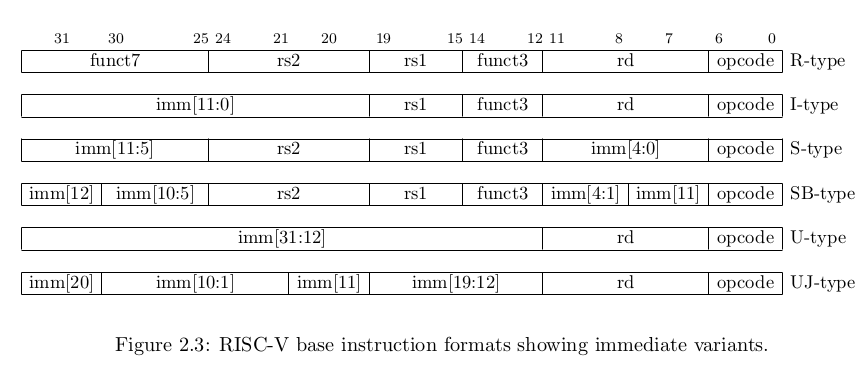
\includegraphics[width=\textwidth]{img/riscv_instructions_format.png}
    \caption{Instruction formats}
    \label{fig:formats}
\end{figure}

\subsection{Pipeline structure}
From an architectural point of view, the design is based on the classic RISC 5-stage pipeline, divided as follows:
\begin{enumerate}
    \item Instruction fetch (IF): the new instruction if read from the instruction memory, pointed by the current Program Counter (PC).
    \item Instruction decode (ID): operands are read from the register file (RF), the control unit generates control signals for the following stages, immediate fields are extended on 32 bits and the ALU controls are decoded.
    \item Execute (EX): the ALU performs the required operation and the new PC is computed in case of branch or jump.
    \item Memory access (DMEM): the data memory is read or written for instructions that require so (load and stores), otherwise data just bypasses this stage.
    \item Write back (WB): either the ALU result or the data memory output is written to the destination register, when required.
\end{enumerate}

Pipeline registers separating each stage take the name of the two stages they are in between (e.g. ID/EX). Actually, assuming a synchronous memory interface, two of these registers are in part bypassed by the memory timing, in order to keep the number of stages at five. For more details on this matter, refer to section \ref{sec:memory}.

The following sections describe the different datapath and control blocks and the testing methodology.

\section{Datapath}
\subsection{Register file}
The RISC-V register file is composed of 32 registers, each 32-bit wide (for RV32I), called \texttt{x0} to \texttt{x31}, where \texttt{x0} is a special register hardwired to the value 0, which can turn useful for some instructions. Figure \ref{fig:rf} shows the top level diagram of the register file structure.

\begin{figure}[hbtp]
    \centering
    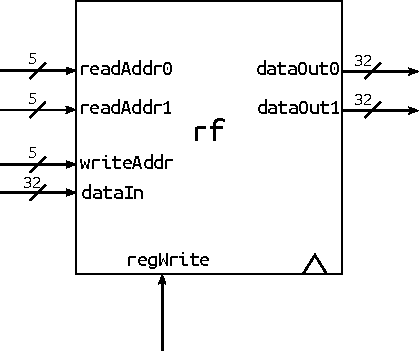
\includegraphics[scale=1]{../register_file/ref/schematic/register_file.pdf}
    \caption{Register file}
    \label{fig:rf}
\end{figure}

Writes to the register file are, of course, synchronous and happen on the positive edge of the clock. For a correct write operation, the destination register must be selected using the \texttt{writeAddr} port, the input data must be placed on the \texttt{dataIn} port and the signal \texttt{regWrite} must be asserted. Internally, the register file will enable only the selected register using a decoder.

Reads are instead combinational and can occur on two different registers at a time, thanks to two different read ports. To select the correct output value, a 32-to-1 multiplexer is used on each read port. However, in order to avoid data hazards during the write back stage, the register file also implements bypassing of input data directly to the output if the same register is read and written during the same clock cycle. Figure \ref{fig:rf_read} shows this read selection process (no multiplexer is used to select 0 in case the register being read is \texttt{x0} as we can suppose it is hardwired directly at its output).

\begin{figure}[hbtp]
    \centering
    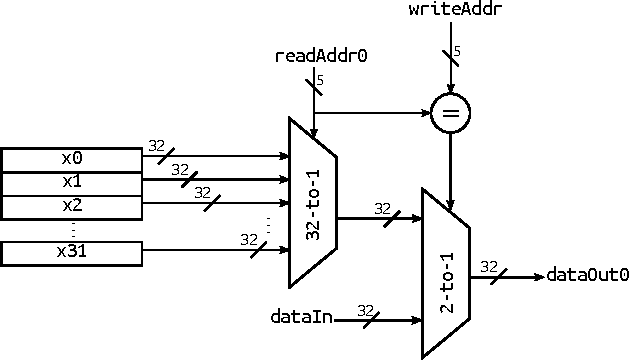
\includegraphics{../register_file/ref/schematic/register_file_deep.pdf}
    \caption{Read operation in the register file}
    \label{fig:rf_read}
\end{figure}

To better illustrate the behavior of the register file operations, their timing diagram is shown in \ref{fig:rf_timing}.

\begin{figure}[hbtp]
    \centering
    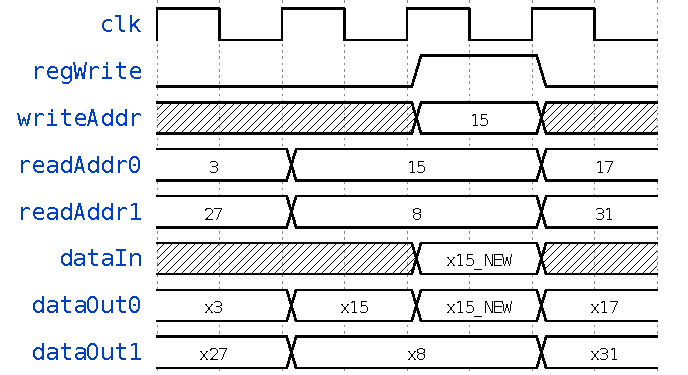
\includegraphics[scale=.8]{../register_file/ref/timing/rf_timing.pdf}
    \caption{Register file timing}
    \label{fig:rf_timing}
\end{figure}

\subsection{ALU}
The ALU is in charge of performing all operations required by arithmetic and logic instructions, load and store, and branch comparison. Figure \ref{fig:alu} shows its top level block diagram, which is simply composed of two inputs and one output on 32 bits, along with a 4-bit control signal to select the desired operation.

\begin{figure}[hbtp]
    \centering
    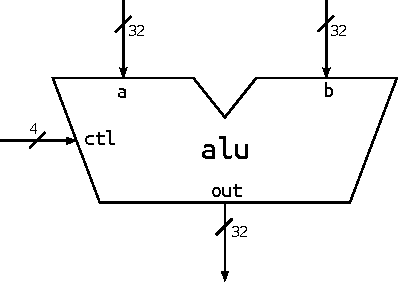
\includegraphics[]{../alu/ref/schematic/alu.pdf}
    \caption{ALU}
    \label{fig:alu}
\end{figure}

The complete list of operation that the ALU can perform is the following (in the order in which they are defined on the \texttt{ctl} input):
\begin{enumerate}
    \item Add
    \item Subtract
    \item AND
    \item OR
    \item XOR
    \item Left shift
    \item Right shift
    \item Right shift with sign extension
    \item Set if equal
    \item Set if not equal
    \item Set if less than
    \item Set if greater or equal than
    \item Set if less than unsigned
    \item Set if greater or equal than unsigned
    \item AUIPC (add current PC and left-shifted immediate)
\end{enumerate}

Note that all operations were described behaviorally as per specifications, in order to be as implementation independent as possible and open to every optimization that a synthesis tool can perform.

All `set if *' operations set the output to the value 1 (\texttt{0x00000001}) if the condition is true, or 0 otherwise. This approach was chosen instead of using flags (such as Carry, Overflow, Negative and so on) to compute conditions as it was deemed simpler to implement and thorough enough, given that there would not have been other uses for the flags.

\subsubsection{ALU decoder}
The control input of the ALU is generated by a special decoder starting from the opcode, funct3 and funct7 fields of each instruction which requires an ALU operation, as described in figure \ref{fig:alu_dec}. This block consists only of a series of conditional statements (that can easily be mapped to multiplexers) which select the correct control signal.

\begin{figure}[hbtp]
    \centering
    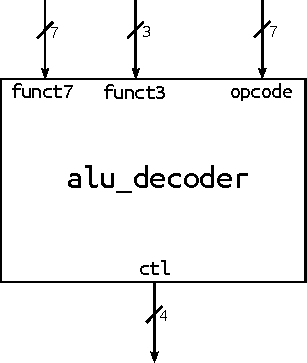
\includegraphics[]{../alu/ref/schematic/alu_dec.pdf}
    \caption{ALU decoder}
    \label{fig:alu_dec}
\end{figure}

Another approach would have been to split the control of the ALU into two decoding steps\footnote{As suggested in Chapter 4 of D. Patterson, J. Hennessy, \emph{Computer Organization and Design RISC-V Edition}, Morgan Kaufmann, 2017}, but a preliminary analysis concluded that no practical advantage would be obtained this way.
Moreover, only few bits of the input fields are required to make a definite decision on the control output, but in order to keep modularity and continuity in the design, the whole fields are given in the interface of the block.

\subsection{Branch and Jump management}
A general view of the unit is given in figure \ref{fig:brJump_man_HW}, along with the significant datapath blocks involved.

\begin{figure}[hbtp]
    \centering
    \makebox[\textwidth][c]{
        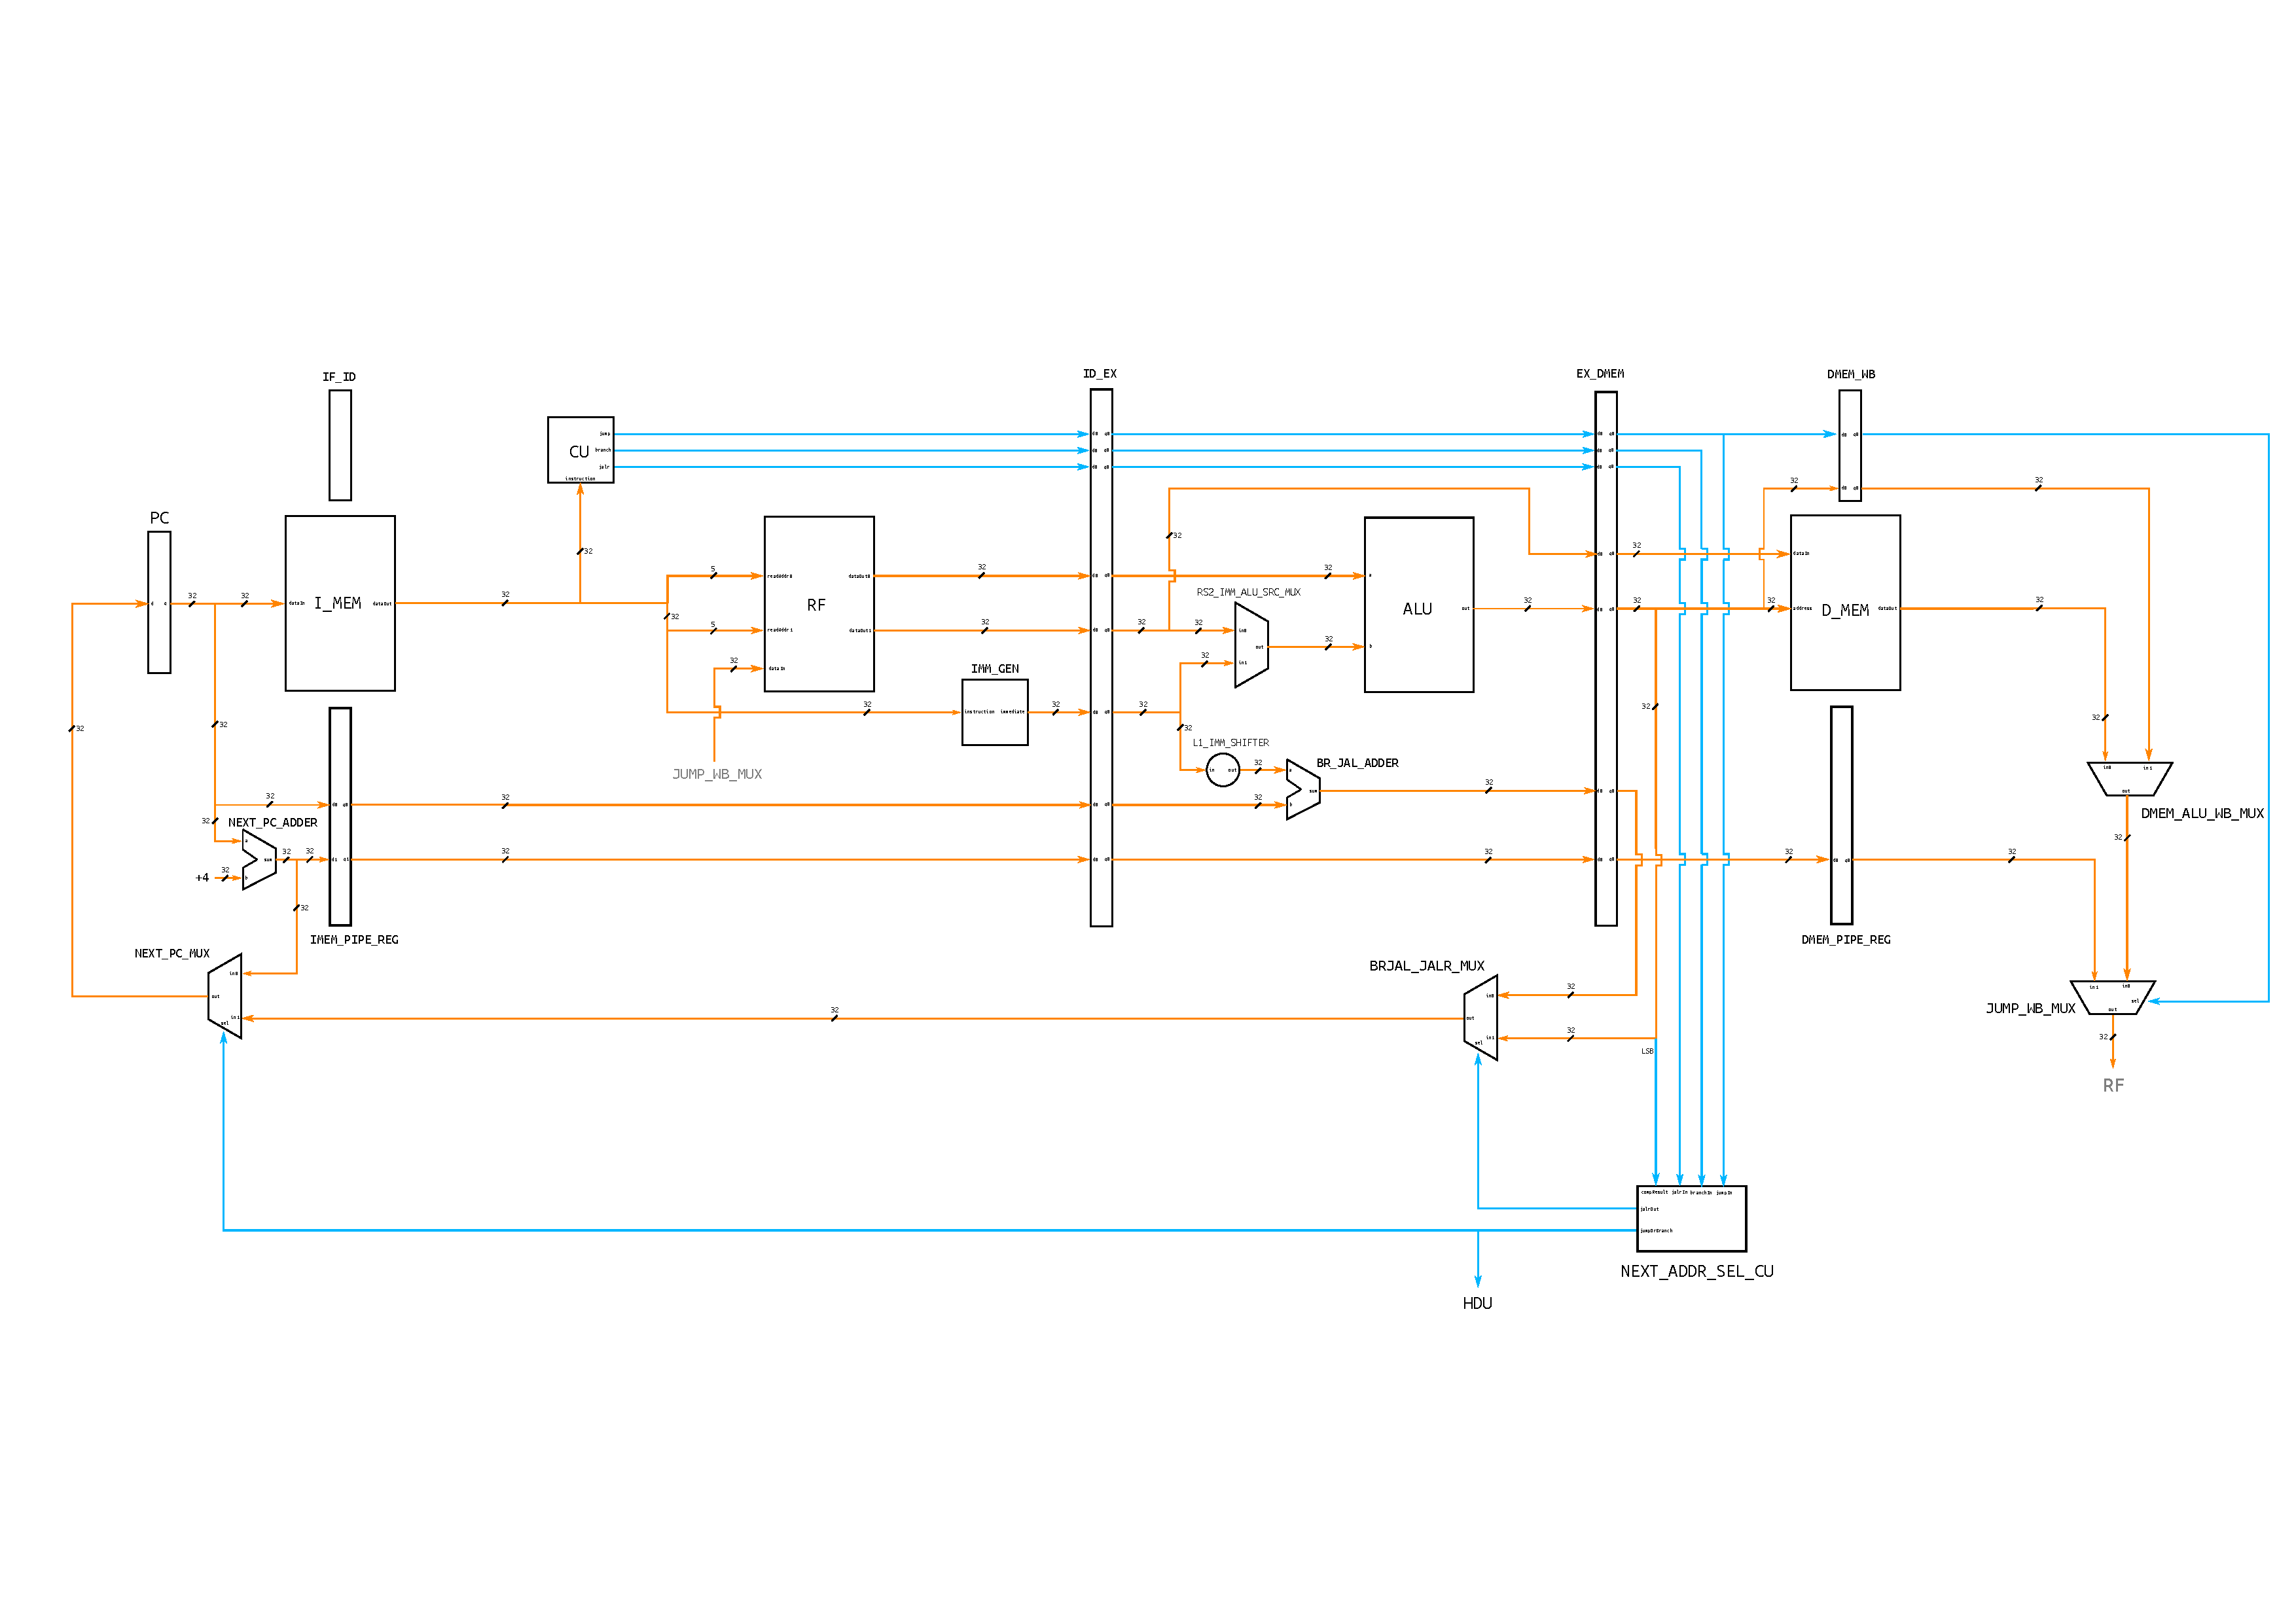
\includegraphics[width=1.2\textwidth]{../br_jmp_management/ref/schematic/branchJump_management_schematic_5stages.pdf}
    }
    \caption{Branch and Jump management HW}
    \label{fig:brJump_man_HW}
\end{figure}

\subsubsection{Types of instructions}
There are two classes of instructions which can lead to a modification of the sequential flow of the program. In the RV32I ISA they are:
\begin{enumerate}
	\item Branches
	\item Jumps
\end{enumerate}
The former is a conditional change of the usual choice of the next address to be put in the PC, whereas the latter is unconditional. The condition, whenever present, is always based on the result of an ALU comparison.

\paragraph{Branch} instructions exist in different flavours, depending on which comparison has to be performed between the content of two registers. Here follows a list of all of them:
\begin{enumerate}
	\item BEQ (branch if equal)
	\item BNE (branch if not equal)
	\item BLT (branch if less than)
	\item BGE (branch if greater or equal than)
	\item BLTU (branch if less than unsigned)
	\item BGEU (branch if greater or equal unsigned)
\end{enumerate}
All these instructions belong to the B-type ones (figure \ref{fig:formats}). They have an immediate field split along the word, which indicates an effective immediate divided by two. Indeed, with a RISC-V standard architecture it is possible to address this way an halfword at most, but never the single byte.
The effective immediate is calculated with a bit reorganization, a sign extension and a left shift of one position, to reach the final 32-bit width.

The instruction contains also the addresses of two registers, whose content will be compared by the ALU to decide whether to take the branch or not.
To distinguish which type of comparison is needed, it is necessary to know the instruction field funct3.

\paragraph{Jump} instructions can be of two types, each bringing to a different hardware path for the data:
\begin{enumerate}
	\item JAL
	\item JALR
\end{enumerate}
\textbf{JAL} is a J-type instruction, whereas \textbf{JALR} is an I-type one. This difference is reflected on the hardware implementation, more on this later.
A jump instruction is unconditional, but still need for an address computation. This operation is different for the two instructions: for JAL it is sufficient to use the same hardware used for branch address computation, whereas JALR requires the non shifted immediate to be added to the content of a register (the next address is not derived by the current one).

\subsubsection{Instruction execution}
Since no \textbf{BPU} (\textbf{B}ranch \textbf{P}rediction \textbf{U}nit) is present in the design, a "branch not taken" assumption is always made when the content of the PC is updated and the decoded instruction is a branch. The simplest way to manage a branch is to delay the decision until the execution stage, waiting for the ALU to do the comparison. The effective decision is then taken in the DMEM stage, not to exacerbate a path which can be critical by itself.
Also the calculation of the next address, which involves the immediate and the program counter, is performed in the execution stage.

A possible improvement could be to anticipate the comparison and the next address calculation in the decoding stage, but to keep the design simple the first solution was chosen, as this would imply additional hardware.
This is compliant with the calculation of the address for a JAL instruction. It is worth to mention that the absence of a condition to be verified is enough to simplify the anticipation of the address calculation and bring it in the decode stage. However this solution would increase the number of resources if the other branch/jump instructions are still executed in an another stage.

A JALR instruction behaves in a slightly different way: the address calculation is performed by the ALU, because the immediate is added to the content of a register.

A branch instruction has no side effects once it has been executed. On the contrary, a jump instruction leaves inside the pipeline the next instruction address to be saved in a destination register. This is not a issue though, because it is possible to see that even without forwarding units no data hazards can arise. If the pipeline was longer, maybe the forwarding unit would be the only thing to have the day saved (the design has it, though).

\subsubsection{Effective calculation}
The address calculation in case of branches/jumps is performed in the execution stage and it depends on the type of instruction:
\begin{itemize}
    \item Branch/JAL: it is based on the "current" PC value (e.g. current for the instruction in that stage). The immediate is sign extended, one position left shifted and added to the PC value (percolated through the pipeline until there) by means of another adder. In the meantime, if the instruction is a JAL, the address of the next instruction goes on through the stages.
    \item JALR: it involves a sum between an immediate and the content of a register. The ALU performs this operation without shifting the immediate. When the result has to be used, the LSB is substituted with a zero. Even in this case, the address of the next instruction follows its path towards the write-back stage.
\end{itemize}

\subsubsection{Next address selection CU}
To control the multiplexers for the next address selection, there's the need for knowing:
\begin{enumerate}
	\item Whether the instruction in the DMEM stage is a branch or a jump.
	\item Which is between the two.
	\item The result of the comparison.
	\item If the instruction is a JALR.
\end{enumerate}
The main CU generates two signals \texttt{branch} and \texttt{jump} which percolate along the pipeline, to allow the ``Next address selection CU" to solve the first two points. The result of a comparison is simply the LSB of the ALU result.
The main CU thus has to generate another signal \texttt{jalr} to indicate a JALR instruction.

The \texttt{jump} control signal is used also in the write-back stage, to select the right input for the register file. If a jump is performed, the data to be written in the destination register is the "next" address after the jump instruction.

In any case, the IMEM pipe register, together with IF/ID, ID/EX and EX/DMEM ones, have to be flushed. This brings to a performance loss of 4 instructions for each taken branch or executed jump.

For details about the \texttt{NEXT\_ADDR\_SEL\_CU}, refer to figure \ref{fig:next_addr_sel_cu} and \ref{fig:next_addr_sel_cu_internalLogic}.

\begin{figure}[hbtp]
    \centering
    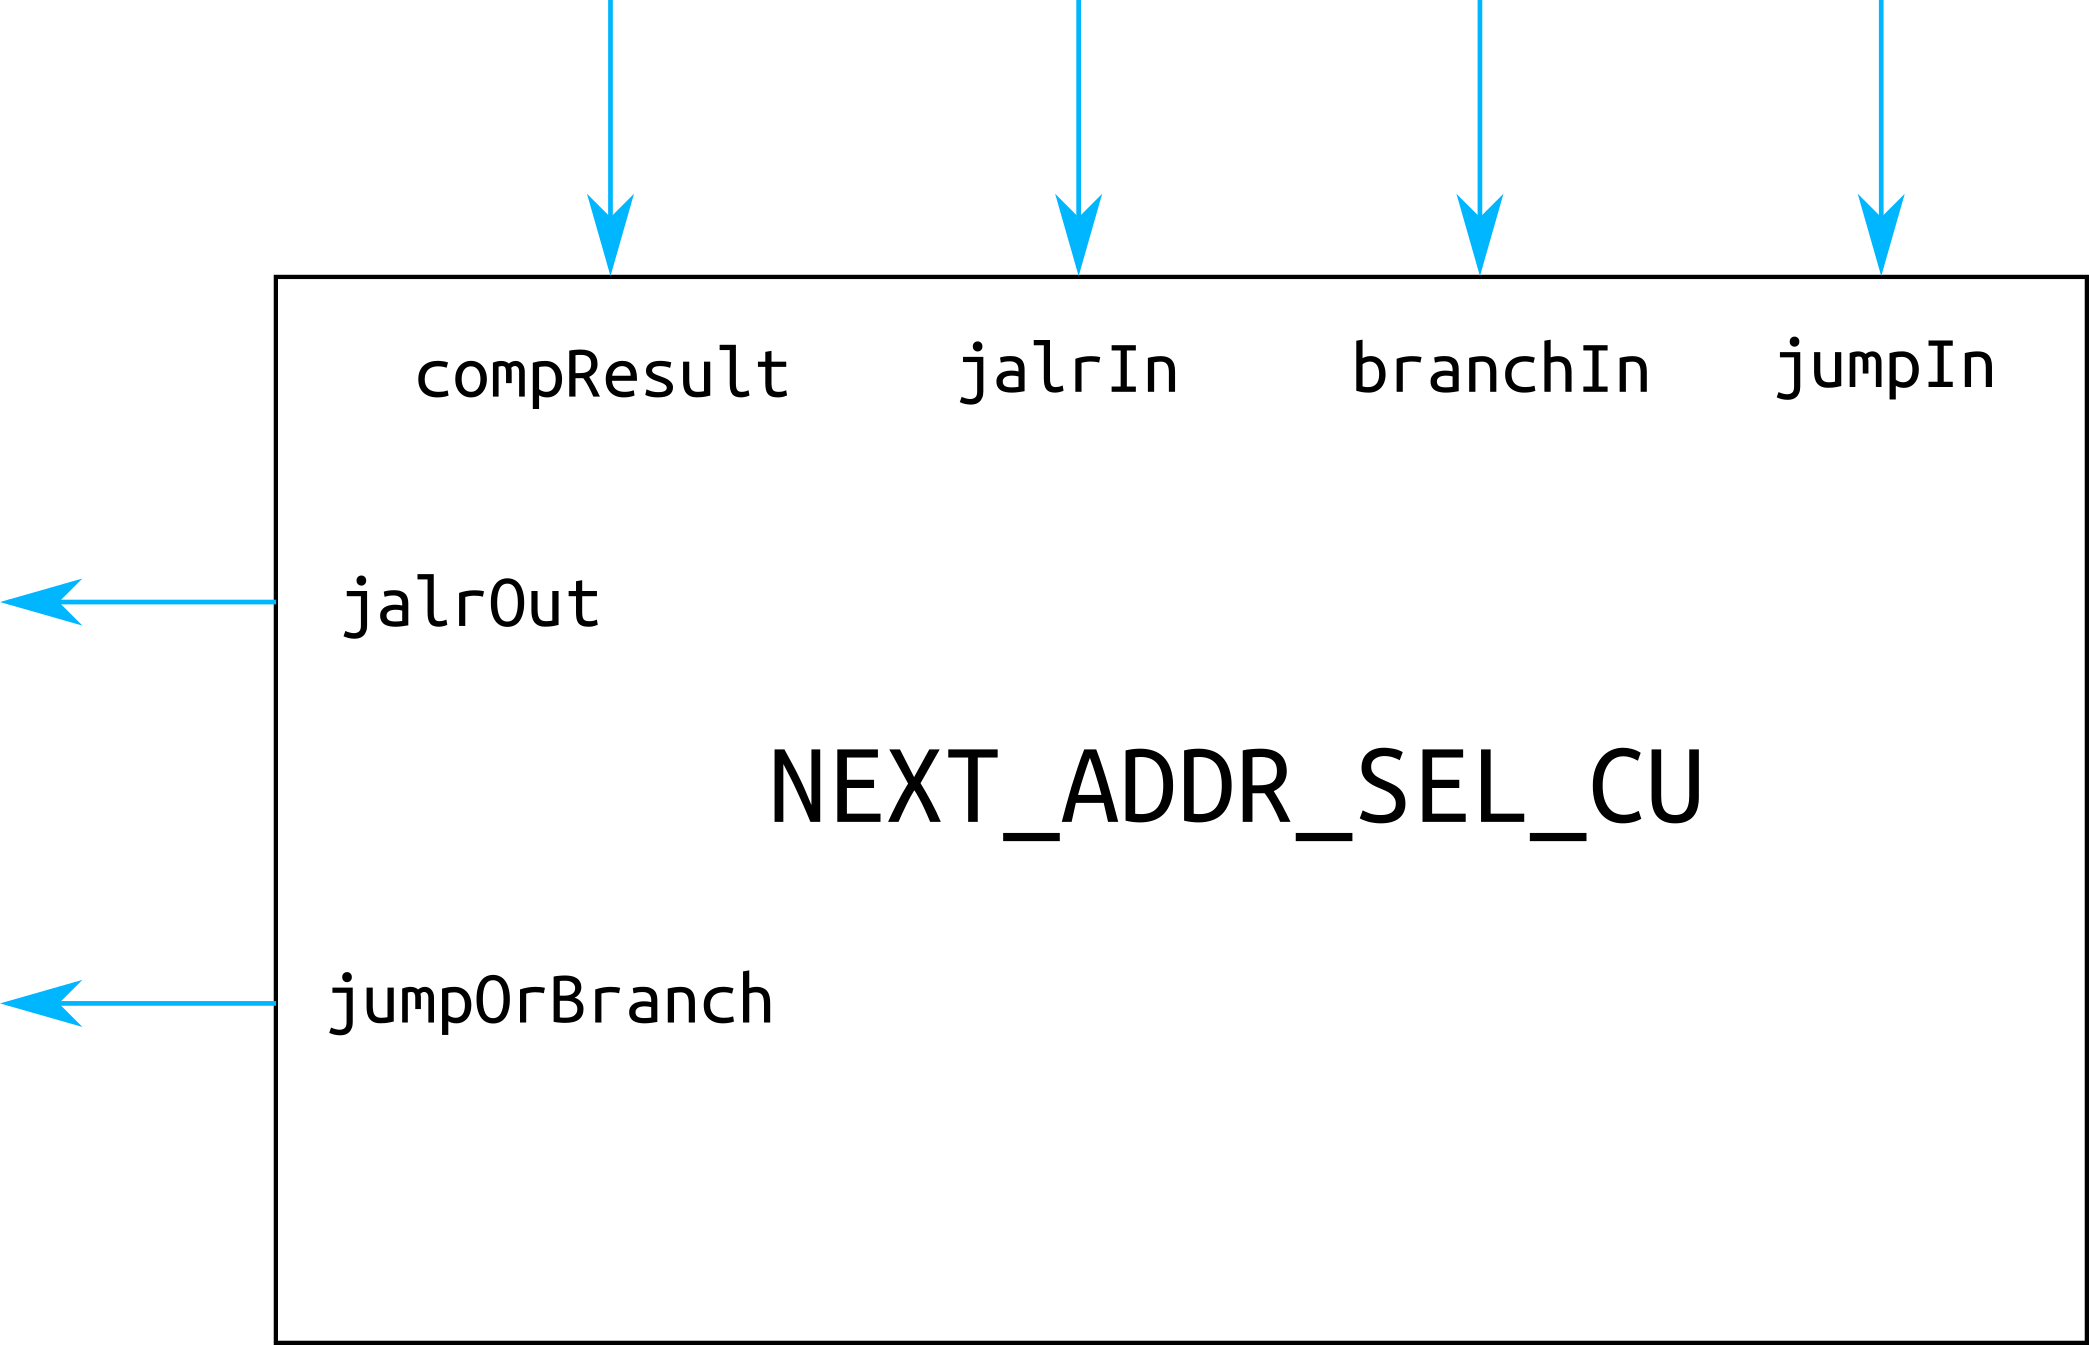
\includegraphics[scale=0.5]{../next_addr_sel_cu/ref/schematic/next_addr_sel_cu.png}
    \caption{Next address selection CU, for jumps and branch management}
    \label{fig:next_addr_sel_cu}
\end{figure}

\begin{figure}[hbtp]
    \centering
    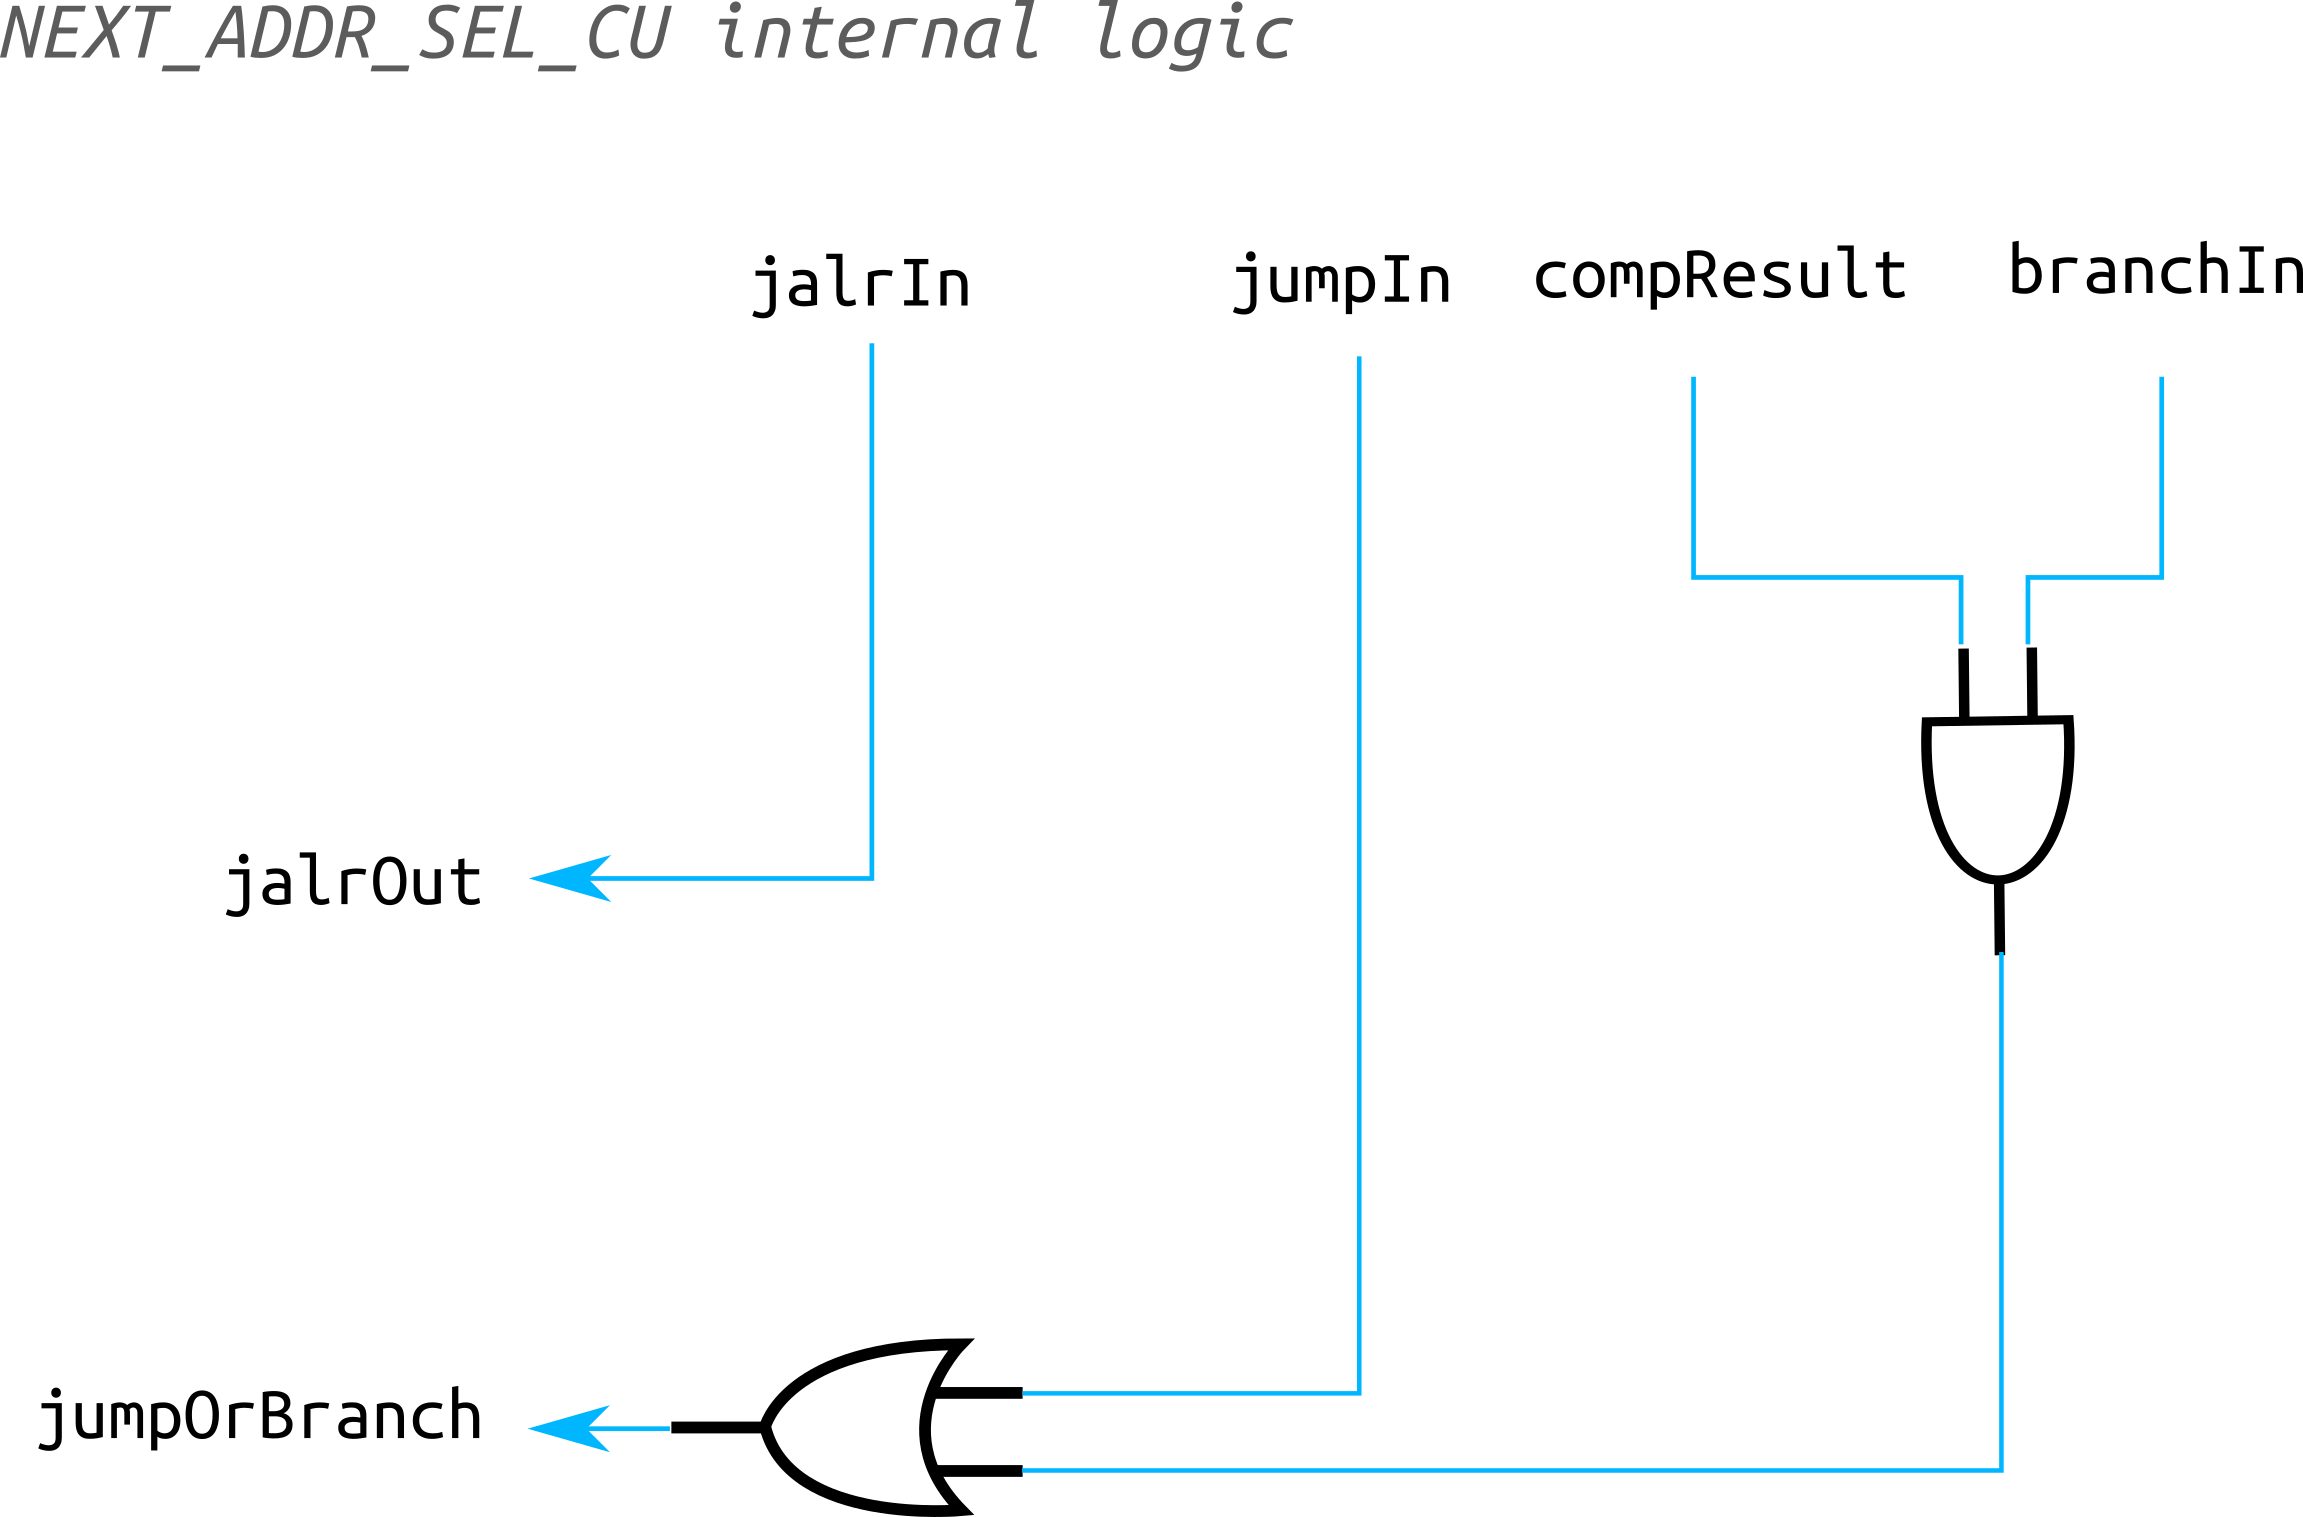
\includegraphics[scale=0.4]{../next_addr_sel_cu/ref/schematic/next_addr_sel_cu_internalLogic.png}
    \caption{Next address selection CU internal logic}
    \label{fig:next_addr_sel_cu_internalLogic}
\end{figure}

\subsubsection{Next address generation}
The next address is chosen by means of two multiplexers:
\begin{itemize}
    \item \texttt{BRJAL\_JALR\_MUX} takes in input the result of the ALU with the LSB masked and the output of the additional adder of the execution stage. These two input come from the EX/DMEM pipe register.
    \item \texttt{NEXT\_PC\_MUX} takes in input the output of \texttt{BRJAL\_JALR\_MUX} and the current PC + 4
\end{itemize}

\section{Control}
\subsection{Forwarding Unit (FWU)}

\begin{figure}[hbtp]
    \centering
    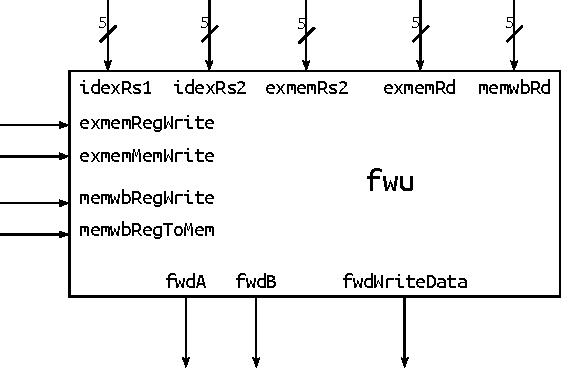
\includegraphics[]{../fwu/ref/schematic/fwu.pdf}
    \caption{Forwarding Unit}
    \label{fig:fwu}
\end{figure}

Forwarding allows to avoid stalling the pipeline when a data hazard occurs between two subsequent instructions, if the needed data is already available in a following pipe stage.
In this five stage pipeline results are written to the destination register during the write back stage, three clock cycles after the operand read in the decode stage. This means that, if an instruction modifies a certain register, only instructions starting from the third after the original would read the correct new data, or equivalently that up to two bubble should be inserted in case of a data hazard.

Forwarding simply bypasses data to the beginning of the execution stage (i.e. at the ALU inputs) if the required results are already present at the ALU output or in the following memory access stage.

To do so, the logic of the FWU (figure~\ref{fig:fwu}) performs some checks:
\begin{itemize}
    \item Check that the earlier in the pipe actually modifies some register (\texttt{regWrite} is asserted) and that the address does not point to register \texttt{x0}.
    \item Compare the destination register in the EX/MEM stage with both source register in the ID/EX stage and, if there is a match, drives the selection signal of the corresponding ALU input multiplexer to select the previous ALU output (\texttt{fwdA/fwdB} $= 10$).
    \item Otherwise, compare the destination register in the MEM/WB stage with both source register in the ID/EX stage and, if there is a match, drives the selection signal of the corresponding ALU input multiplexer to select the result currently in the memory access stage (\texttt{fwdA/fwdB} $= 01$).
\end{itemize}

Note that, according to the list above, forwarding gives precedence to data present in the EX/MEM stage over the MEM/WB stage if the same register is present in both, as the former contains the latest result.

\subsubsection{Load/store forwarding}
The designed forwarding unit handles also the another special case of data hazard that occurs when a load is followed immediately by a store to the same memory location, such as in memory to memory copies.

In this case the FWU checks that the two involved instructions are actually a load (\texttt{memToReg} asserted in the MEM/WB stage) and a store (\texttt{memWrite} asserted in the EX/MEM stage) and that the destination and source registers are the same, and if that is the case drives the control of the multiplexer selecting the memory data input to choose the memory output.

Figure \ref{fig:fwu_5stages} shows the FWU with all inputs on which decisions are taken and the three output signals controlling the related multiplexers in each pipeline stage of the core.

\begin{figure}[hbtp]
    \centering
    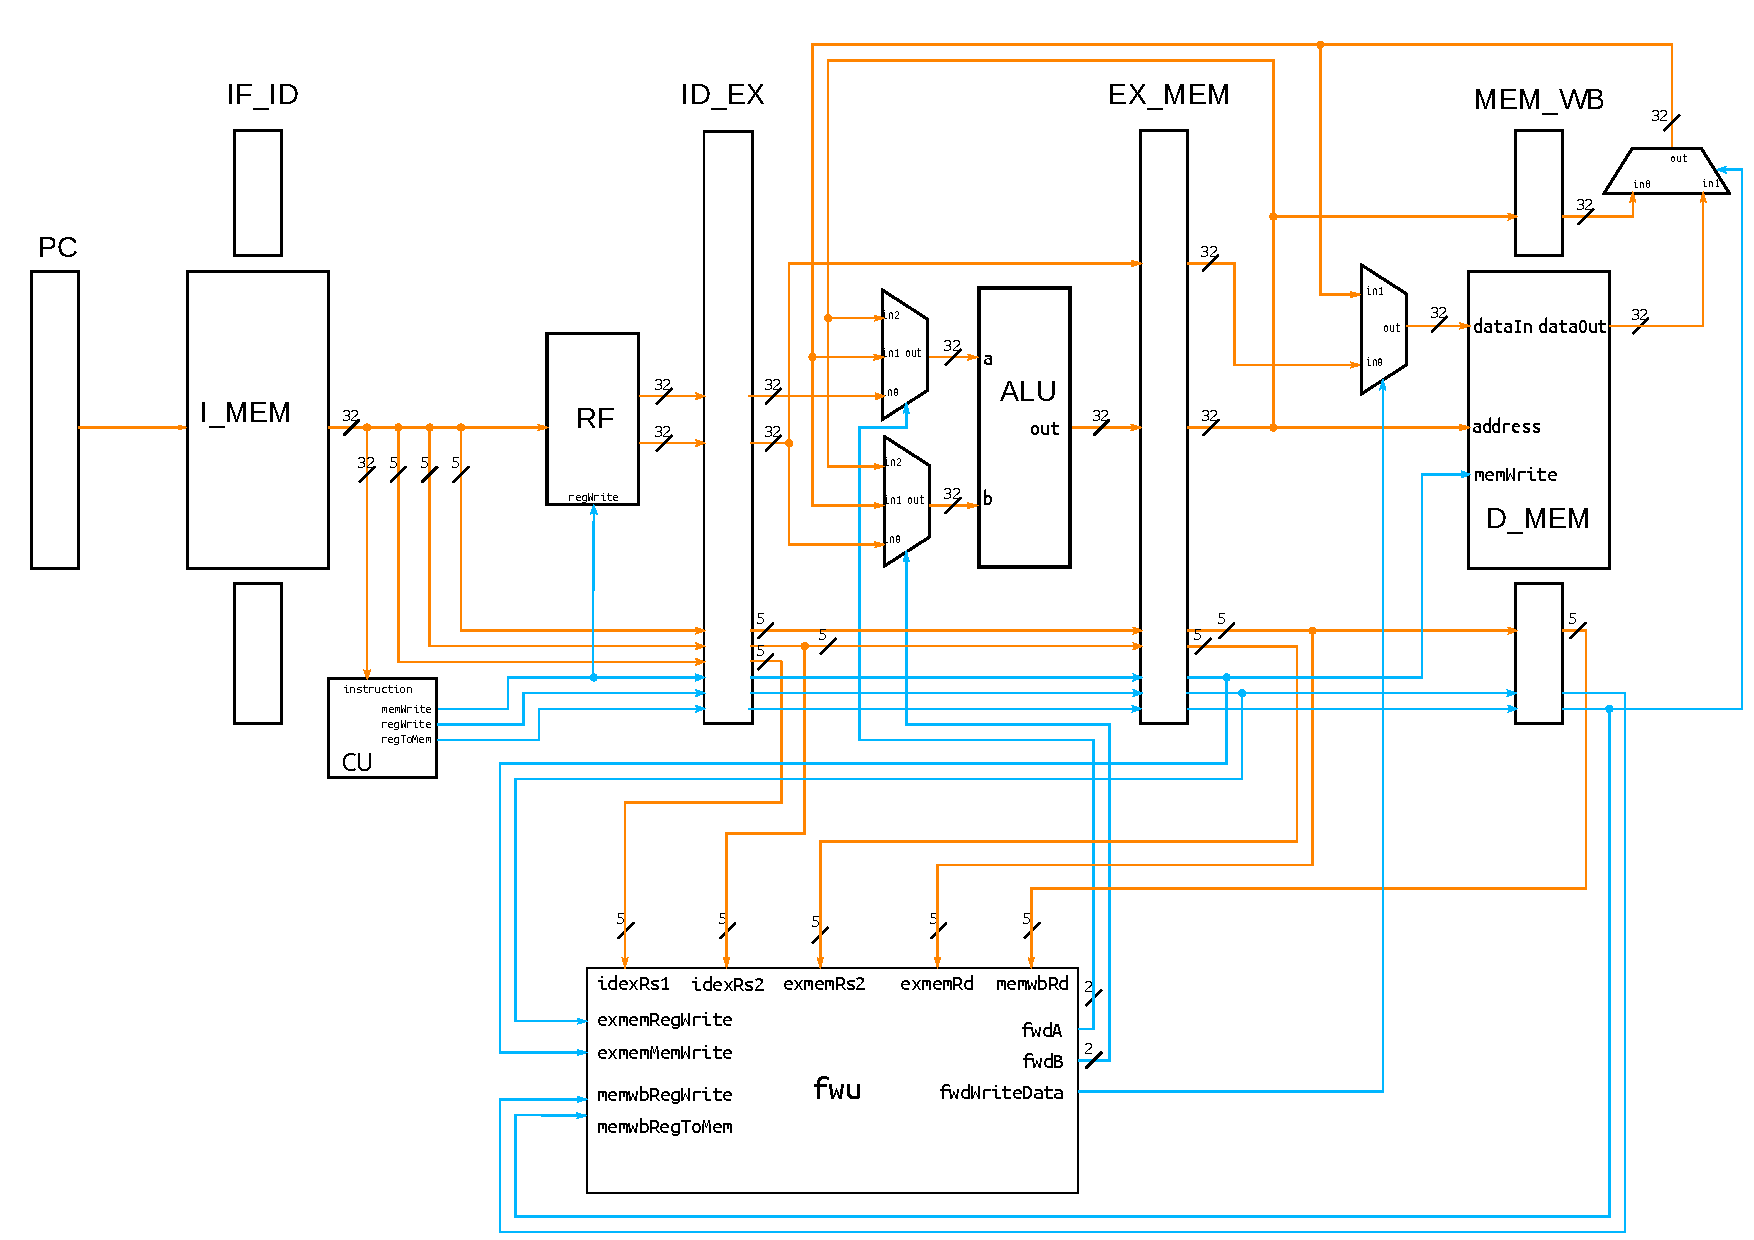
\includegraphics[width=\textwidth]{../fwu/ref/schematic/fwu_5stages.pdf}
    \caption{Forwarding Unit connection to the datapath of the core}
    \label{fig:fwu_5stages}
\end{figure}

\subsection{Hazard Detection Unit (HDU)}
When data cannot be forwarded, then the pipeline must be inevitably stalled by preventing the fetch of a new instruction and inserting a bubble. Specifically, this happens when a data hazard occurs between a load (\texttt{memRead} asserted in the decode stage) and another using instruction (unless it is a store, for which forwarding accounts).

Moreover, when a branch is taken or an unconditional jump occurs, a similar action of flushing the entire pipeline to get rid of invalid instructions already in execution must be taken.

Both this occurrences are handled by the Hazard Detection Unit (figure \ref{fig:hdu}), that according to the aforementioned checks, outputs three signals:
\begin{itemize}
    \item \texttt{stall\_n}: active low, is connected to the enable of the Program Counter and the IF/ID pipe register to prevent them from changing in the event of a stall.
    \item \texttt{flushIdEx}: to drive the multiplexer inserting the NOP in the ID/EX register, that will propagate to the rest of the pipeline, in case of a stall or a jump.
    \item \texttt{flushIfIdExMem}: to drive the multiplexer inserting the NOP in the IF/ID and EX/MEM registers in case of jump.
\end{itemize}

\begin{figure}[hbtp]
    \centering
    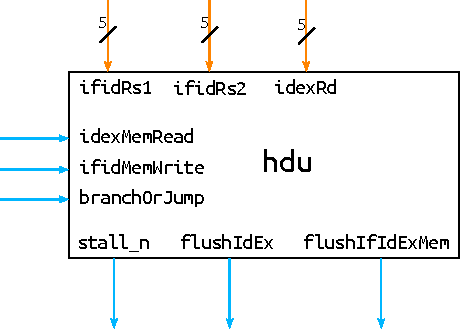
\includegraphics[]{../hdu/ref/schematic/hdu.pdf}
    \caption{Hazard Detection Unit}
    \label{fig:hdu}
\end{figure}
A summary of the possible cases when this can occur is reported in table \ref{tab:hdu_output}:

\begin{table}[hbtp]
\centering
\begin{tabular}{|c|c|c|c|}
\hline
                        & \texttt{stall\_N} & \texttt{flush\_IdEx} & \texttt{flush\_IfId\_ExDmem} \\ \hline
\textbf{No Hazard}      & 0                          & 0                             & 0                                     \\ \hline
\textbf{Control Hazard} & 0                          & 1                             & 1                                     \\ \hline
\textbf{Data Hazard}    & 1                          & 1                             & 0                                     \\ \hline
\end{tabular}
\caption{HDU output}
\label{tab:hdu_output}
\end{table}

\subsubsection{Inserting a NOP}
The NOP instruction is not present in the RISC-V ISA. It is possible to emulate it though, using an \texttt{ADDI x0 x0 0}. This instruction does nothing, because the register x0 is hardwired to value 0. The instruction NOP belongs to the set of pseudo-assembly instructions: they are translated in RISC-V language on the fly by the assembler, and they exist for programmers ease only.

For an effective NOP insertion in the IF/ID stage there is the need for a sequential control of the multiplexer which drive the source of the RF. There is no way of doing it before the pipe register, unless a NOP instruction is already present somewhere in memory.

In figure \ref{fig:hzd_management} a high level datapath for hazard management is depicted. Moreover, a timing diagram to show how instructions are flushed is shown in figure \ref{fig:hzd_management_timing}. The three instructions which follow a jump or a taken branch are discarded.

\begin{figure}[hbtp]
    \centering
    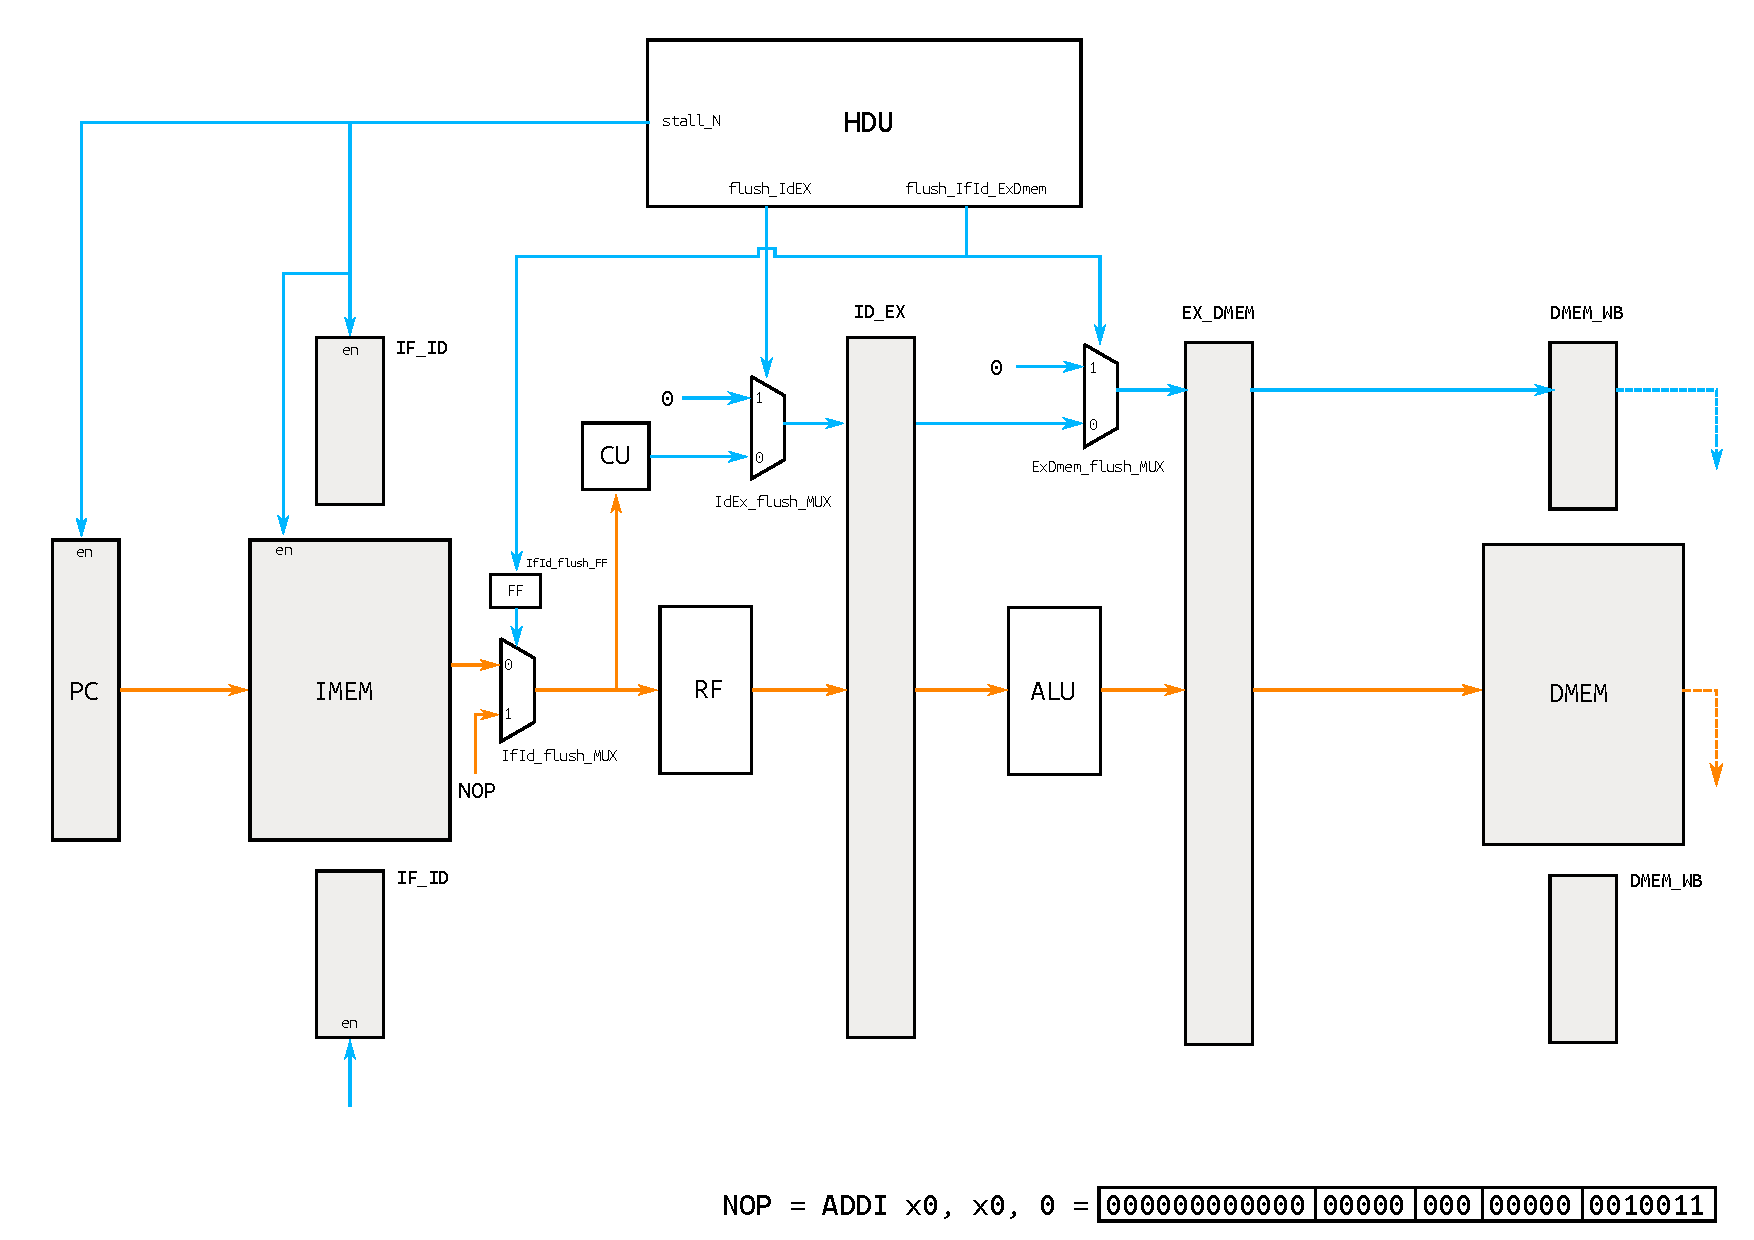
\includegraphics[scale=0.5]{../hzd_management/ref/schematic/hzd_management.pdf}
    \caption{Hazard management HW}
    \label{fig:hzd_management}
\end{figure}

\begin{figure}[hbtp]
    \centering
    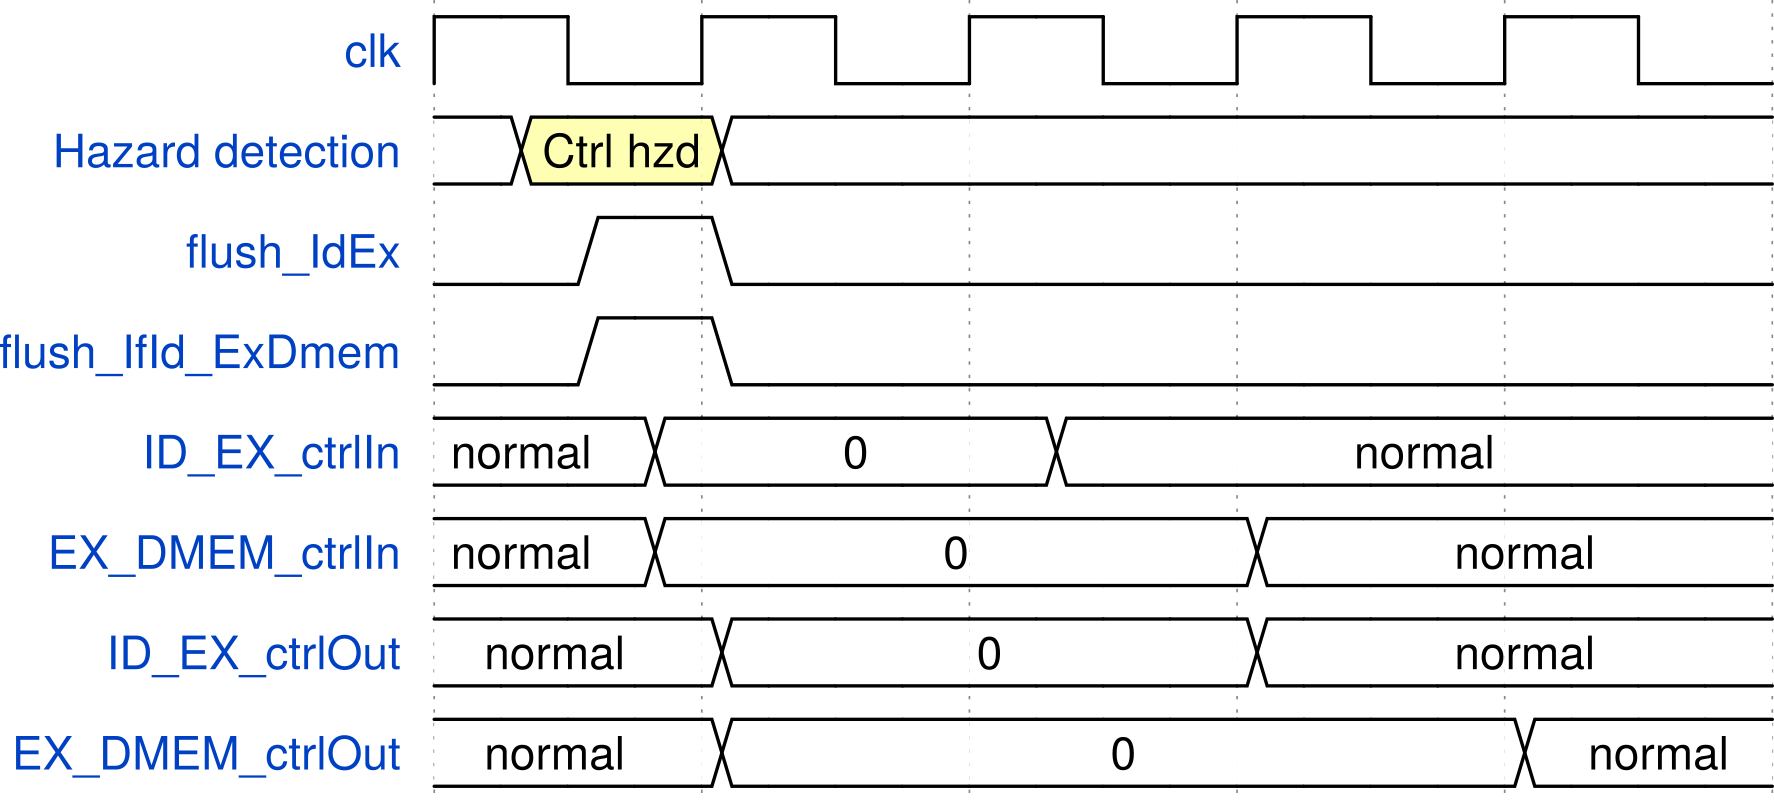
\includegraphics[scale=0.8]{../hzd_management/ref/timing/hzd_management_timing.png}
    \caption{Hazard management timing}
    \label{fig:hzd_management_timing}
\end{figure}

\subsection{Control Unit (CU)}

\begin{figure}[hbtp]
    \centering
    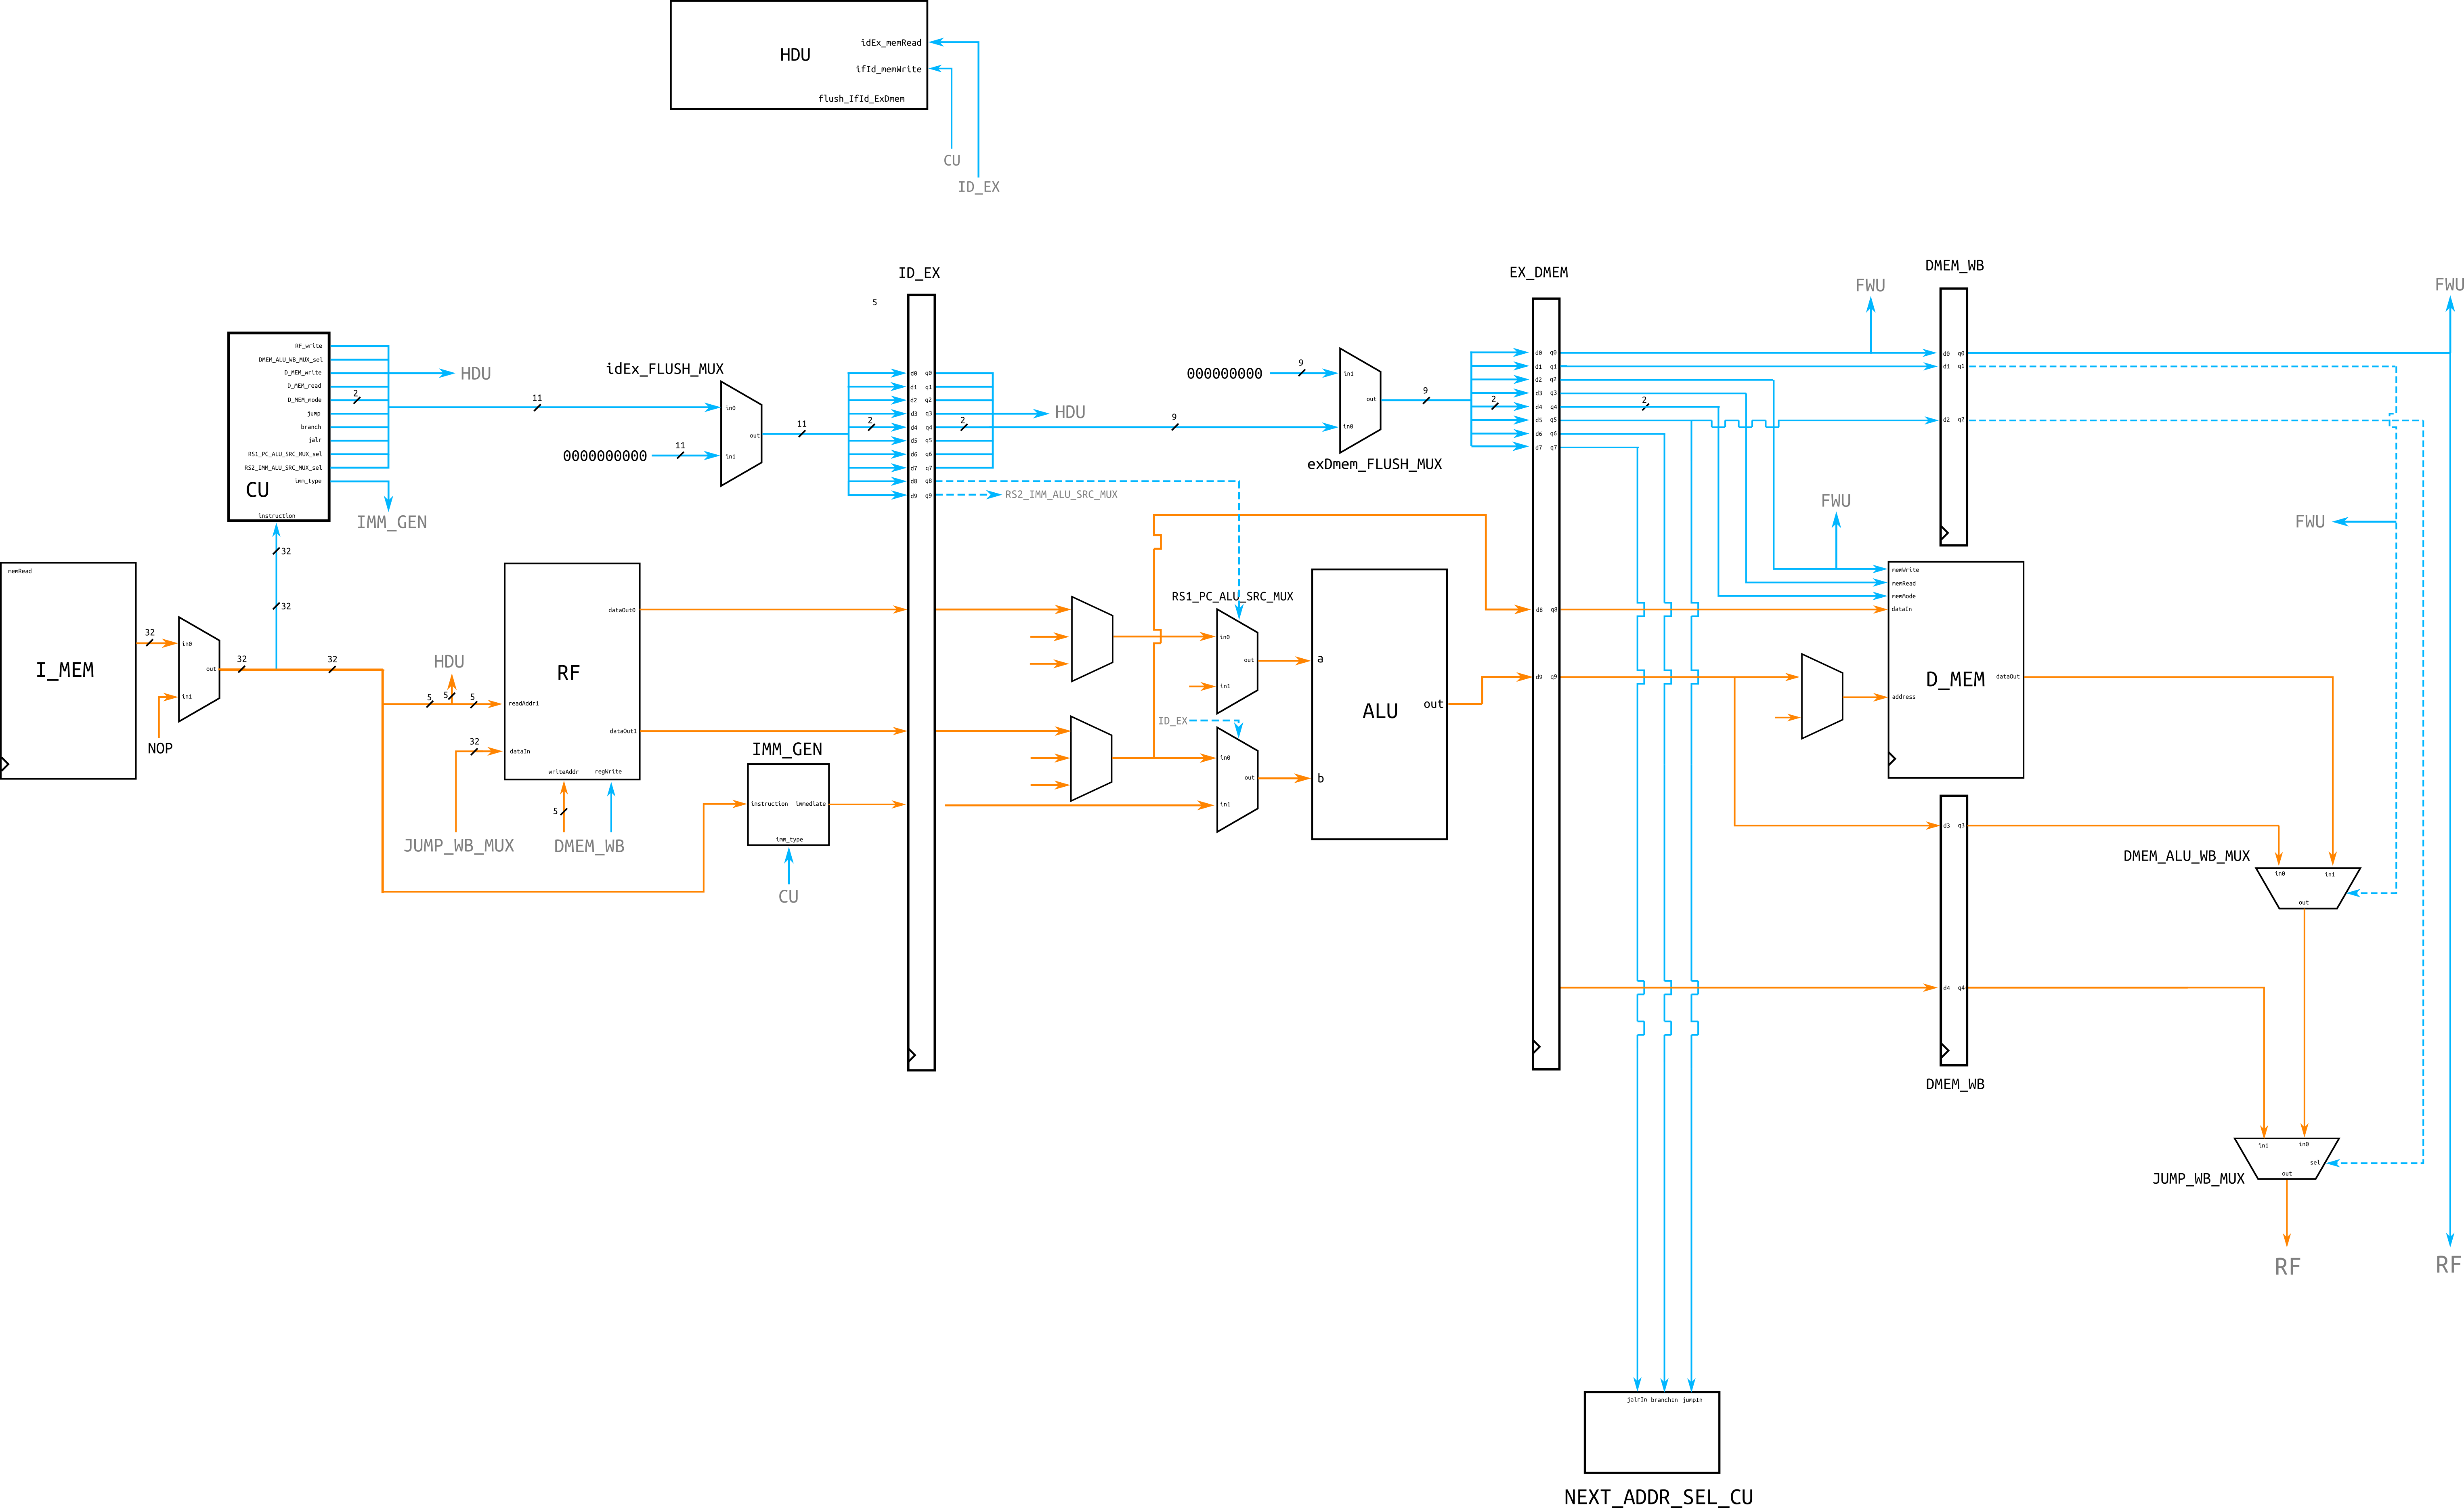
\includegraphics[scale=0.3]{../cu/ref/schematic/cu.png}
    \caption{Control Unit and the units connected to it}
    \label{fig:cu}
\end{figure}

The Control Unit is shown in figure \ref{fig:cu}. It is a combinational component, because all the synchronization is done in the pipeline registers. It basically reads the opcode and other eventual flags (funct3, funct7) to determine the format of the instruction used in the immediate generator, as well as other flags.

These flags are about memory commands (read, write, how much to read/write), register-file commands (write, address is generated in the remaining datapath), MUX commands (to decide the inputs to use for the ALU) and branch/jump commands.

There are two commands which are a bit less standardized, to tell the memory the dimension to access (byte, halfword, word) and to tell apart the different jump conditions like branch, jal, jalr.

It is implemented in a behavioral way, to avoid possible risks, and all the parameters are defined as constants, to be easily updated if needed.

\subsection{Immediate Generator (ImmGen)}

\begin{figure}[hbtp]
    \centering
    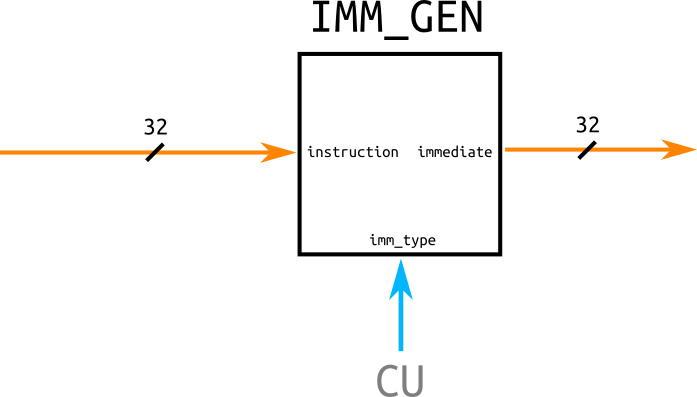
\includegraphics[]{../immgen/ref/schematic/immgen.png}
    \caption{Immediate Generator}
    \label{fig:immgen}
\end{figure}

The Immediate Generator (show in figure \ref{fig:immgen}) is needed to gather the correct bits from the different instruction formats. The type of instruction is signalled by the Control Unit, and the output is the reconstructed immediate in the same cycle, since it is a combinational component.

\section{Main architecture}
The main architecture is depicted in figure \ref{fig:rv-magic_main}. One multiplexer was added in the execution stage to add the support for the AUIPC operation.

\begin{figure}[hbtp]
	\centering
    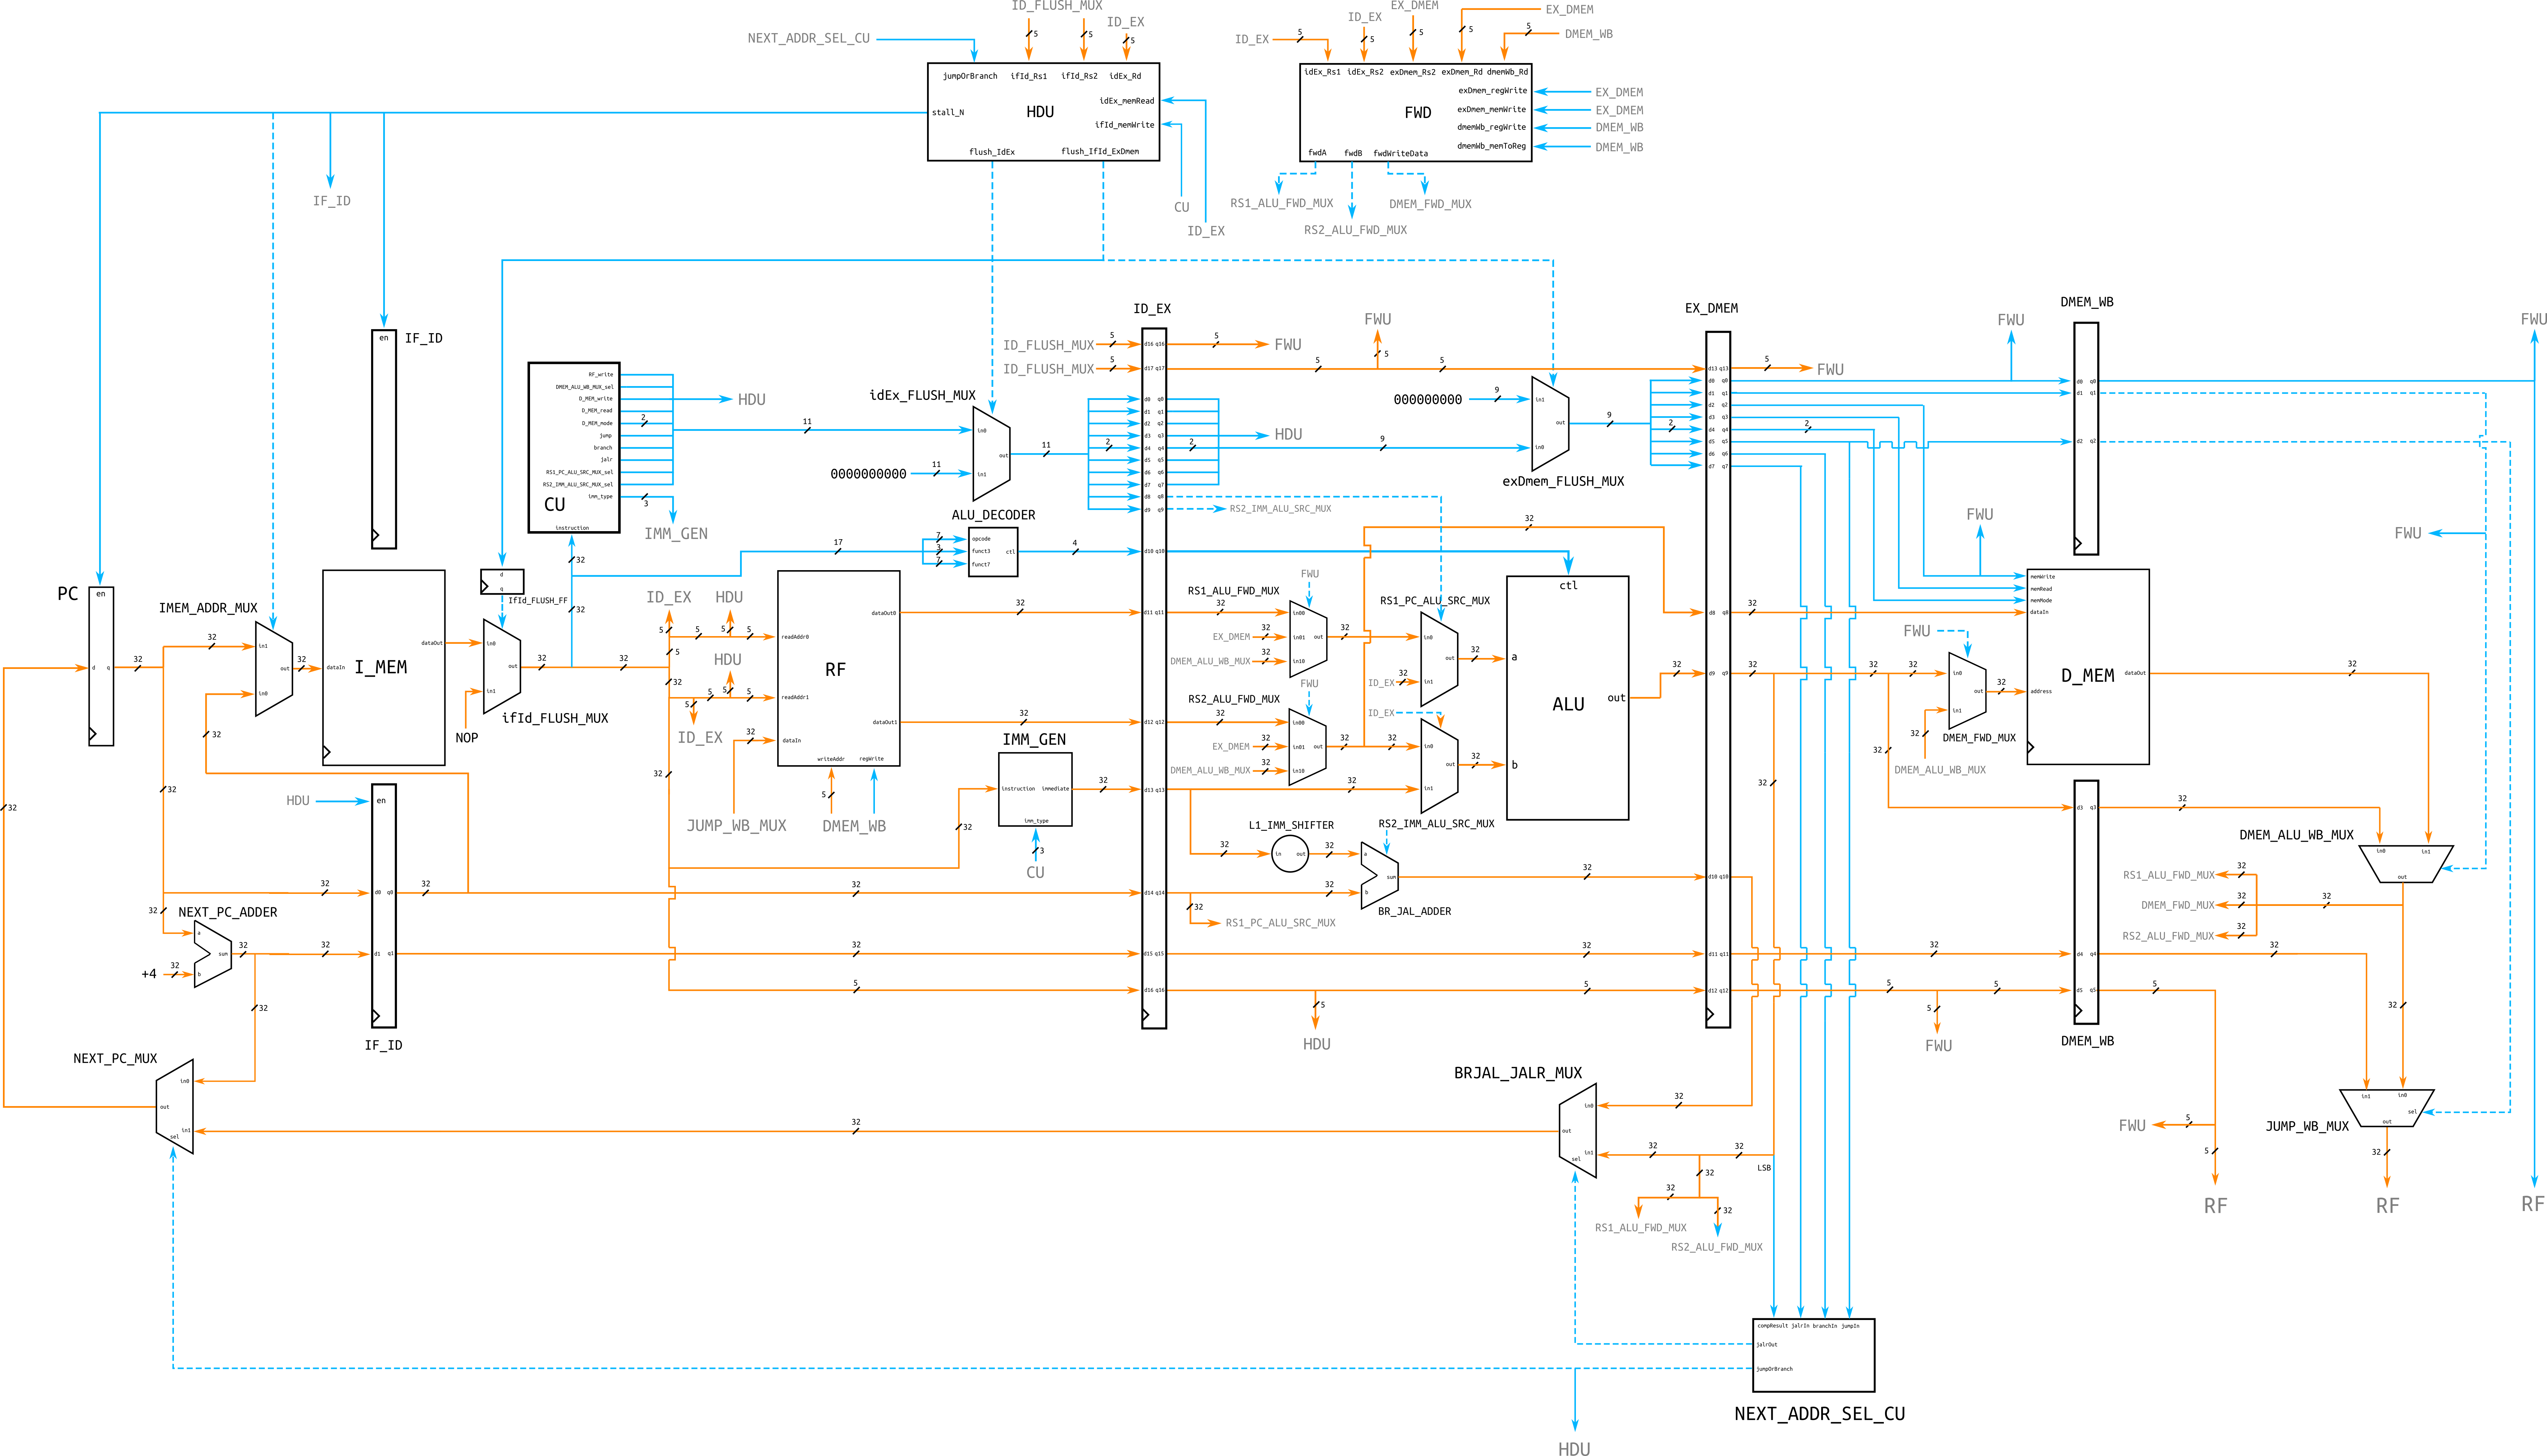
\includegraphics[scale=0.2]{../main/ref/schematic/rvMagic.png}
    \caption{RV-MAGIC main architecture}
    \label{fig:rv-magic_main}
\end{figure}

\section{Testbench}
\subsection{Memory}\label{sec:memory}
Some kind of memory model is needed in order to perform a full simulation of the processor core. Given that the design of a full fledged memory subsystem is beyond the scope of this experience, we resorted to a simple behavioral model of a synchronous memory.

This model is only intended for simulation purposes and does not map a real memory chip on its own, but emulates the function of a more complex memory controller able to select individual bytes among a 32-bit word both in read and in write operations.

Figure \ref{fig:memory} shows the interface of this block, where the \texttt{address} is left parametric, as it can differ between instructions and data memory. Note that compliant to the RISC-V byte addressing specification, each address represents a single byte, even if the data width is always 32 bits, which is the width of the data bus of the architecture. The data width for load and stores is selected by the \texttt{addrUnit} signal, according to the following encoding:
\begin{itemize}
    \item 00: byte
    \item 01: halfword (16 bits)
    \item 10: word (32 bits)
\end{itemize}
Independently of the data width chosen, the correct output is always provided within a single clock cycle. It this behavior was to be replicated on a real byte-addressed memory chip, it would take (at most) four read operations and a clock four times faster.

Read and write operations are handled by the couple of control signals \texttt{memRead} and \texttt{memWrite}, of which only one should be asserted at each clock cycle to perform the desired action. Both signals active represent an forbidden condition and should be avoided by the whatever is in charge of controlling the memory.

\begin{figure}[hbtp]
    \centering
    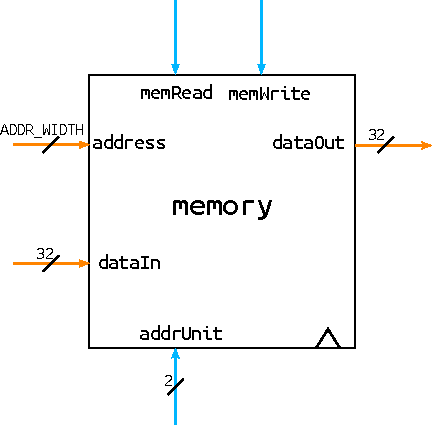
\includegraphics[scale=1]{../memory/ref/schematic/memory.pdf}
    \caption{Memory}
    \label{fig:memory}
\end{figure}

Figure \ref{fig:memory_timing} shows the usual timing diagram of this fully synchronous memory, according to which both reads and writes take place at the next clock cycle after the proper control signals are asserted.

\begin{figure}[hbtp]
    \centering
    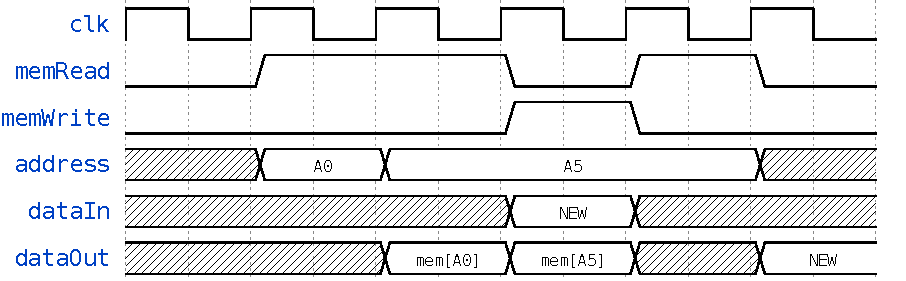
\includegraphics[scale=.8]{../memory/ref/timing/memory_timing.pdf}
    \caption{Memory timing diagram}
    \label{fig:memory_timing}
\end{figure}

\subsection{Main}\label{sec:main}
To test the whole processor, some patterns of instructions were develped. The main purposes were to check:
\begin{enumerate}
\item the correct behaviour of each instruction in a flow without hazards
\item the correct management of all the hazards
\end{enumerate}
To achieve this in an easier way, an assembler was developed to support a translation from the RISC-V assembly to the machine code. A detailed discussion about this tool is provided in section \ref{sec:assembler}. Initially a search on the net was done to find a toolchain to convert high level languages like C in RV32I instructions, but a lot of issues arose and another strategies were chosen. The developing of an assembler is not critical, because of its static nature: it works like a decoder and it does not need to be "clever" like a compiler. Testing needs weren't critical and a string check-processing was enaugh.

\paragraph{Instructions}

\paragraph{Testbench} The testbench was written in Verilog coherently with all the previous work. The entity instantiates the \textbf{DUV} (\textbf{D}evice \textbf{U}nder \textbf{V}erification) together with the two memories. It also handles the clock and reset generation.
It is worth to note that the addressable space of the memory was reduced because a complete 32-bit one was not feasable due to space problems: only a subset of the PC bits was bound to the address line of the storage devices.
The entire system is reset at the beginning of the simulation, and a parametric clock is fed to all the sequential elements.
An \textit{initial} statement inside the memory modules ensures the correct loading of the instructions/data inside them. To perform this task, the function \textit{\$readmemh} is used: it allows to read an ASCII text file in which are present hexadecimal data written in rows. Each row is assigned to a vector of the memory.

With the aid of the GUI of Modelsim, each signal was visually followed to check if the timing of the processor was respected. The first tested code is the following:

% ADD THE CODE

The first instructions are LUI to load the RF with positive and negative values. A writing to x0 is performed to verify its immutability.

\subparagraph*{lui x0, 37} Nothing has to be saved in x0, because it is hardwired to gnd.

\subparagraph*{lui x1, 133} The 20 bits immediate \textbf{133} = 00000000000010000101 is sign extended to 32 bits and 12-bits left shifted (with zero padding), then it is brought to the ALU to exit it without any processing. The result is saved to the destination register.
\begin{enumerate}
\item Immediate: 00000000000010000101 = 133
\item Sign extension, left shifting and zero padding: 00000000000010000101000000000000 = 544768
\end{enumerate}
The result is saved in x1.

\begin{figure}[hbtp]
    \centering
    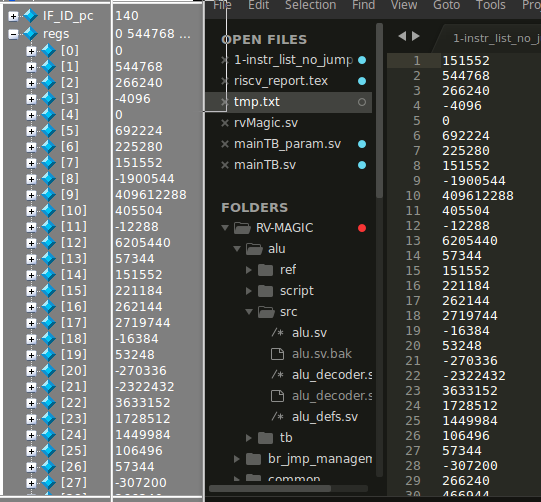
\includegraphics[scale=.8]{/home/matteo/git/RV-MAGIC/main/sim/plot/first_LUIs_validation.png}
    \caption{RF loading verification}
    \label{fig:first_LUIs_ver}
\end{figure}

And so on. At the fetch of AUIPC the PC is equal to $4 \times 32 = 128$. The previous instruction, i.e. the last LUI, is being decoded: for its completion there's the need for waiting for other four cycles. At this point (PC = 144) all the register file were checked to verify the correct storage of the data (figure \ref{fig:first_LUIs_ver}).

\subparagraph*{auipc x2, 6466} The 20 bits immediate \textbf{6466} is sign extended, left shifted and added to the content of the PC relative to the instruction itself (PC = 128).
\begin{enumerate}
\item Immediate: 00000001100101000010 = 6466
\item Sign extension, left shifting and zero padding: 00000001100101000010000000000000 = 26484736
\item Sum with PC: 00000001100101000010000010000000 = 26484864
\end{enumerate}
The result is saved in x2.
The same procedure was followed to verify all the other instructions of the RV32I ISA.

Once all the basic logical/arithmetical functions were verified in this soft way (not all the possible combinations were tested!), jumps and branches were taken into account.

\subsubsection{Assembler}\label{sec:assembler}

\end{document}
